% !TeX root = Report.tex
\documentclass[12pt]{article}

% Package imports (organized and deduplicated)
\usepackage{biblatex}
\usepackage{changepage}
\usepackage{color}
\usepackage{enumitem}
\usepackage{float}
\usepackage{graphicx}
\usepackage{listings}
\usepackage{sectsty}
\usepackage{xcolor}
\usepackage[breaklinks=true]{hyperref}
\usepackage{xurl}
\usepackage{tikz}
\usepackage{lipsum}
\usetikzlibrary{shapes.geometric,positioning,fit,backgrounds}
\usepackage{./timing-diagrams}
\usetikzlibrary{calc}
\setcounter{biburlnumpenalty}{100}
\setcounter{biburlucpenalty}{100}
\setcounter{biburllcpenalty}{100}

% \usepackage{background}
% \backgroundsetup{
%   position=current page.north west,
%   angle=0,
%   nodeanchor=north west,
%   vshift=-1cm,
%   hshift=1cm,
%   color=red,
%   opacity=1,
%   scale=1,
%   contents={Preprint}
% }

\definecolor{darkblue}{RGB}{0, 0, 102} 
\hypersetup{
    colorlinks=true,
    pdfborder={0 0 0},
    linkbordercolor=white,
    urlcolor=darkblue,
    linkcolor=darkblue,
    citecolor=darkblue,
    filecolor=darkblue
}

% Make bibliography ragged right instead of justified
\AtBeginDocument{
  \renewcommand{\bibsetup}{\raggedright}
}
% Document configuration
\restylefloat{table}
\graphicspath{{./images/}}
\addbibresource{Library.bib}
\subsectionfont{\fontsize{12}{14}\selectfont}

% Author information
\author{
    Joar Heimonen\\
    \texttt{contact@joar.me}
}

% Title configuration
\title{
    \textbf{Spark4pi-sensors}\\[0.5em]
    \large Project Plan
}
\date{\today}

\newcommand{\license}{
    \vspace{1em}
    \noindent\small{© 2024 Joar Heimonen\\
    This work is licensed under a \href{https://creativecommons.org/licenses/by-sa/4.0/}{Creative Commons Attribution-Sharealike 4.0 International License}.}
    \vspace{1em}
}

\begin{document}
\maketitle

\begin{abstract}
    \noindent Spark4pi-sensors is a hardware platform for analog, i2c and SPI sensors. 
    This document describes the preliminary hardware schematic and the development plan for the Spark4pi-sensor platform. 
    Spark4pi-sensors implements six RJ45 sensor interfaces based on Sensirons reference implementation. 
    Three different power rails are implemented. Groups of two sensors share one of the four available
    power rails, each group also shares an i2c bus.
\end{abstract}

\pagebreak

\tableofcontents

\pagebreak


\section{Introduction}
When designing a sensor platform, universality is of the highest importance. This document will describe the preliminary implementation of Spark4pi-sensors and the development plan.
Spark4pi-sensors is a hardware platform for analog, i2c and SPI sensors. The platform is designed to support a wide range of sensors powered by a wide range of voltages.
The platform is designed to be rack mounted taking up one unit in a 19" rack. This platform is powered by a 12V power supply our trough PoE using the ethernet4pi-zero PoE hat.
The platform will be controlled and configured through a NETCONF/YANG interface. 


\section{Technical background}
\subsection{Power Over Ethernet (PoE)}
Power over Ethernet (PoE) is a technology that allows network cables to carry electrical power. 
There are two standards for PoE, IEEE 802.3af and IEEE 802.3at \cite{IEEEStandardsAssociation}. The ethernet4pi-zero PoE hat uses IEEE 802.3af which 
is the older standard and allows for a maximum power draw of 15.4w.

\subsection{Raspberry Pi Zero}
The Raspberry Pi Zero is a single board computer developed by the Raspberry Pi Foundation \cite{foundationTeachLearnMake2025}. 
The Raspberry Pi Zero is the smallest and cheapest Raspberry Pi.

\subsection{Ethernet4pi-zero PoE}
The ethernet4pi-zero PoE is a PoE network shield in the late stages of development.
The shield is designed to be used with the Raspberry Pi Zero and the Raspberry Pi Zero W.
Ethernet4pi-zero PoE is built around a Lightside-Instruments powermod-54260 which delivers a maximum of five volts at three amps.
This is equal to a maximum power draw of 15 watts which is the maximum power draw of the IEEE 802.3af standard.

\subsection{Powermod-54260}
The powermod-54260 is a DC to DC voltage regulator that can deliver a maximum of five volts at three amps.
It works with an input voltage between 10 and 60 volts. The powermod-54260 is designed to be modular and
can be placed on any project that requires a stable five-volt power supply. It is based on the Texas Instruments TPS54260 \cite{TPS54260DataSheet}.


\subsection{RJ45}
A RJ45 connector is a type of connector commonly used on Ethernet cables.

\subsection{Sensirion RJ45 sensor interface}
Sensirion uses the RJ45 connector to implement their proprietary sensor interface.
This interface is designed to be used with their reference sensor implementations. Through 
an adapter called the SEK-SensorBridge.

\subsection{YANG}
YANG is a data modeling language, similar to XML. It is used to model and configure the state of network controlled devices \cite{bjorklundYANG11Data2016}
YANG implements a hierarchical model of what the device can do. Unlike SNMP this model is fetched from the device.

\subsection{NETCONF}
NETCONF is a protocol that is used to configure and monitor network devices. It uses the YANG data modeling language to describe the configuration and state of network devices.
NETCONF can be implemented over any protocol but is usually implemented over SSH \cite{ennsNetworkConfigurationProtocol2011}.

\section{Hardware Design}
\subsection{Schematic overview}
\begin{figure}[H]
    \begin{adjustwidth}{-1.5in}{-1in}
        \centering
        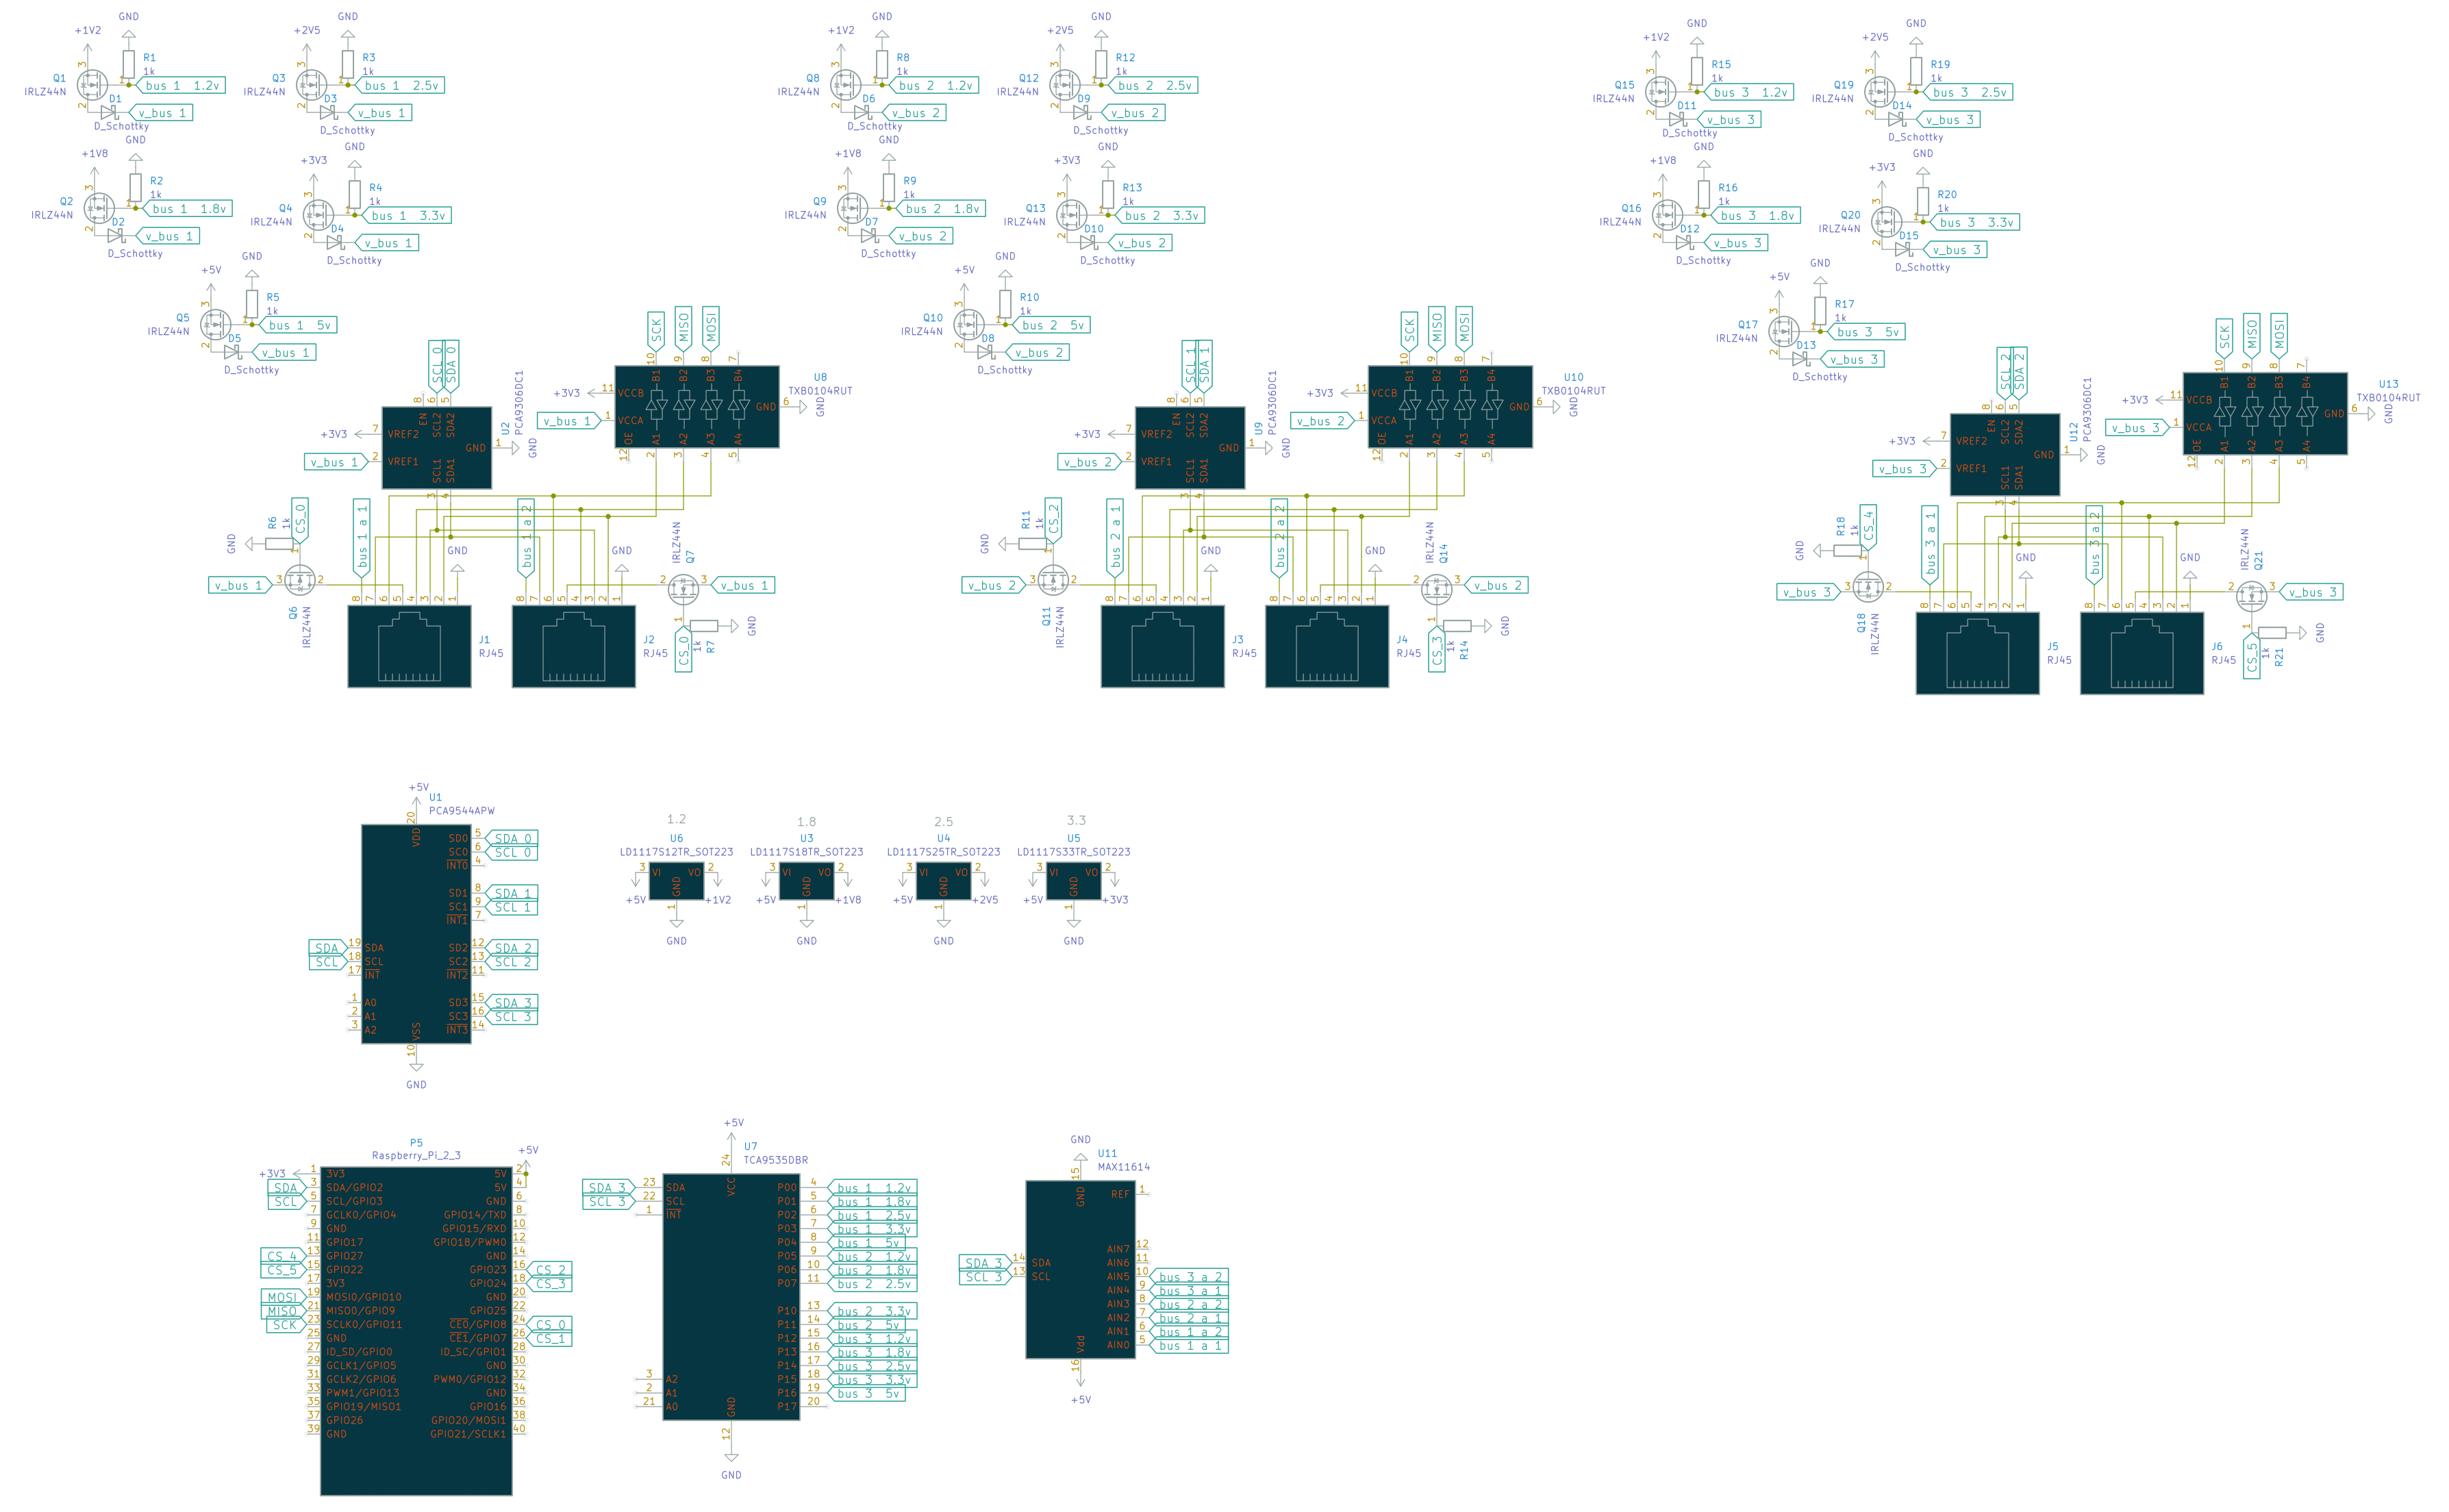
\includegraphics[width=\paperwidth]{spark4pi-sensors-1.png}
        \caption{Preliminary schematic overview of the Spark4pi-sensors platform}
    \end{adjustwidth}
\end{figure}

\subsection{Power distribution}
The Spark4pi-sensors has five power rails for the sensors.
\begin{itemize}
    \item 5V
    \item 3.3V
    \item 2.5V
    \item 1.8V
    \item 1.2V
\end{itemize}
Each power rail except for the 5V is based on the LD1117 voltage regulator. This regulator can output a maximum of 1300mA. With each of 
the Sensirion sensors drawing a maximum of 300 mA this is enough as long as all sensors are not drawing the maximum current from the same power rail.

\subsection{Sensor interfaces}
The Spark4pi-sensors platform has six RJ45 sensor interfaces. Each interface is based on the Sensirion reference implementation.
Each interface consists of a RJ45 connector, a power management system, two level shifters, an i2c bus, an SPI bus and an analog input.
The RJ45 connectors pin-out looks like this:
\begin{itemize}
    \item 1: GND
    \item 2: SCK
    \item 3: SCL
    \item 4: MISO
    \item 5: VDD / Chip select
    \item 6: MOSI
    \item 7: SDA
    \item 8: Analog input
\end{itemize}
The same interface can implement an analog sensor and an i2c and SPI sensor. Due to the VDD ping also functioning as a chip select pin
All SPI operations must be paused when reading from an interface the implements SPI.
\subsection{Busses}
The Spark4pi-sensors platform has four i2c busses and one SPI bus. Each i2c bus is shared between two sensors. The SPI bus is shared between all sensors.
\subsubsection{i2c bus}
To get four i2c busses we are multiplexing our Raspberry PI zero i2c0 bus. We achieve this by using the PCA9544APW i2c multiplexer.
The PCA9544APW is a four-channel i2c multiplexer. It has a single i2c address and can be controlled by the Raspberry Pi.
Here is an overview of the i2c busses:
\begin{itemize}
    \item i2c bus 0: Sensor 1 and Sensor 2
    \item i2c bus 1: Sensor 3 and Sensor 4
    \item i2c bus 2: Sensor 5 and Sensor 6
    \item i2c bus 3: TCA9535DBR 18 channel IO expander and a MAX11614 eight channel ADC
\end{itemize}
Each of the three sensor i2c busses contains a level shifter that is used to shift the i2c from 3.3v to the sensor bus voltage (1.2v, 1.8v, 2.5v, 3.3v, 5v).
\subsubsection{SPI bus}
The Spark4pi-sensors platform has a single SPI bus that is shared between all sensors. This is the Raspberry Pi SPI bus.
The SPI bus uses MOSFET's to enable the VDD pin on the sensors interface when a read or write operation is performed.
When an interface is not in SPI mode the VDD pin will always be enabled.
Each of the dual interface pairs has a level shifter that is used to shift the SPI bus from 3.3v to the sensor bus voltage (1.2v, 1.8v, 2.5v, 3.3v, 5v).
\subsection{Analog input}
The Spark4pi-sensors platform has six analog inputs. Each analog input is connected to a MAX11614 eight channel ADC.
This ADC is connected to the Raspberry Pi through the i2c bus 3. The ADC is used to read the analog sensor connected to the RJ45 interface.
\subsection{Enclosure}
The Spark4pi-sensors platform is designed to be rack-mounted. The platform takes up one unit in a 19" rack.
For illustration purposes, we have included an image of the spark-v2 kit as our enclosure will be similar to this.
\begin{figure}[H]
    \centering
    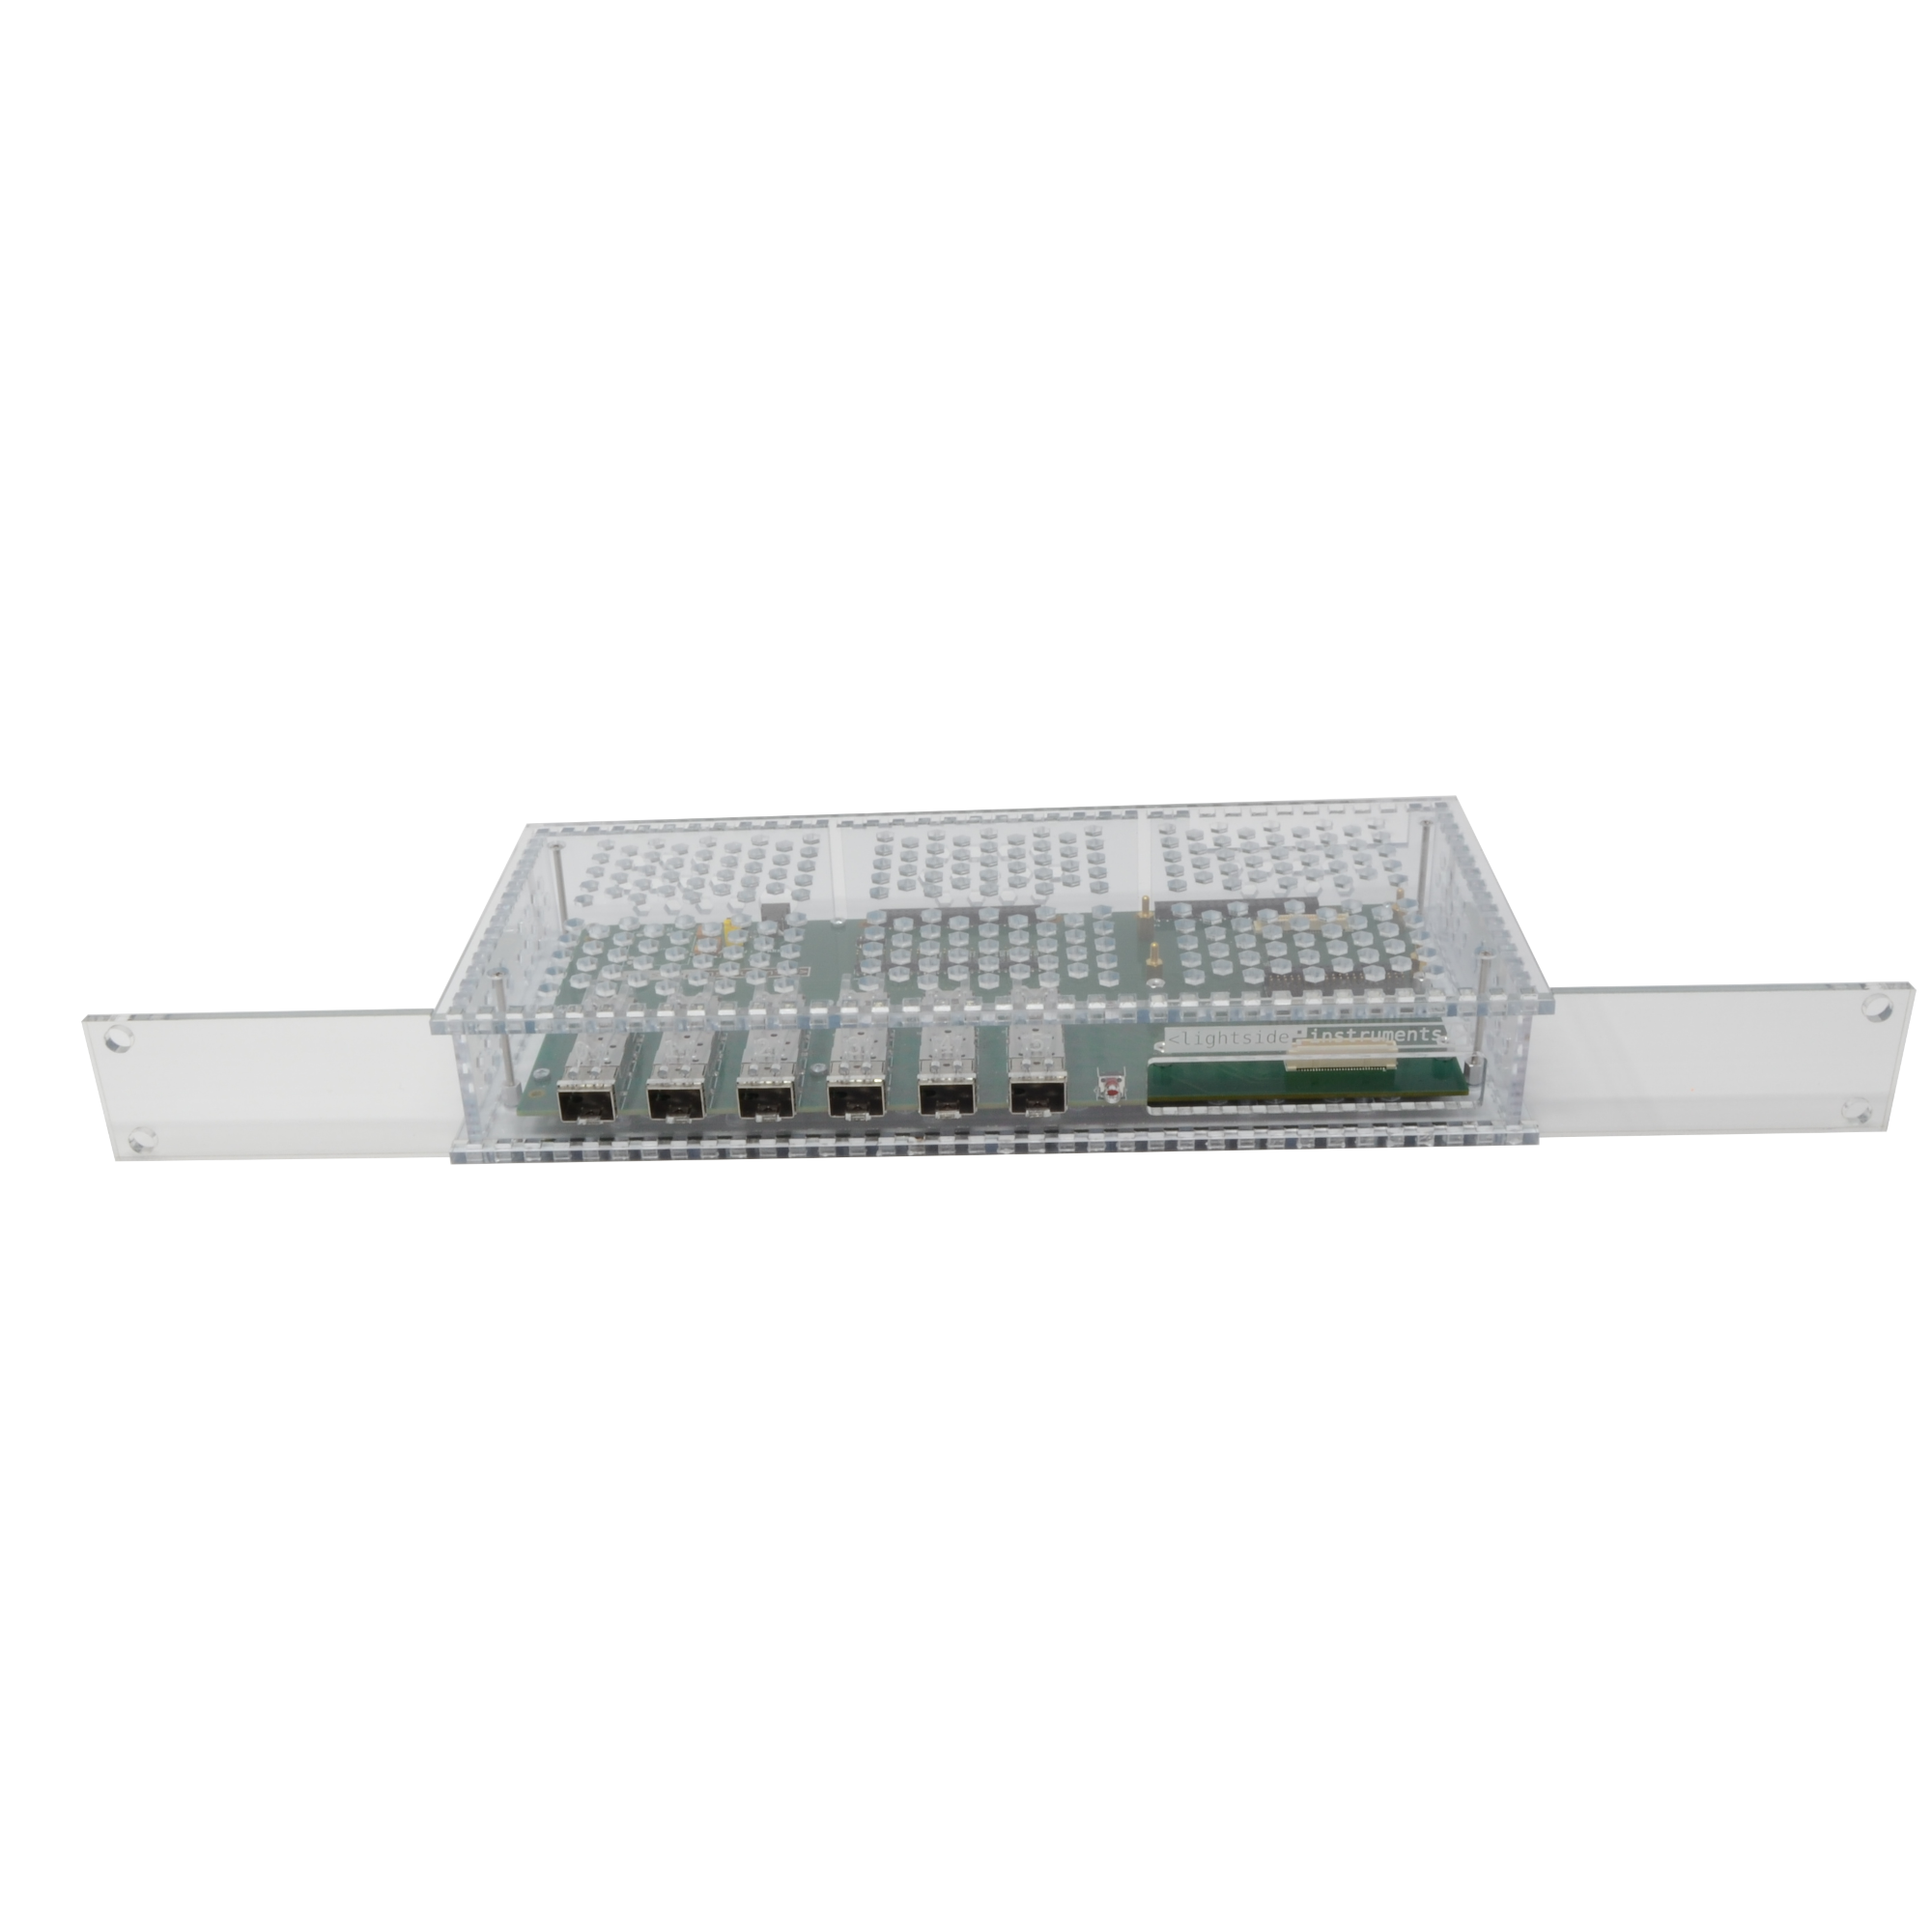
\includegraphics[width=\textwidth]{enclosure.png}
    \caption{Spark-v2 kit}
\end{figure}

\section{Development plan}
The development of this project will be divided into three phases.
\subsection{Phase 1}
\begin{itemize}
    \item Finalize the schematic
    \item Order the PCB's
    \item Debug the PCB's
    \item Repeat until the PCB's are working
\end{itemize}
Whilst waiting for the finalization of the PCB's other members of the team will
work on getting up to speed with the NETCONF/YANG interface, designing the 
YANG model, Auditing our codebase and setting up a build server
\subsection{Phase 2}
\begin{itemize}
    \item Develop an API for controlling the Spark4pi-sensors platform
    \item Develop a YANG model for the Spark4pi-sensors platform
    \item Develop a NETCONF server module for the Spark4pi-sensors platform
\end{itemize}
\subsection{Phase 3}
\begin{itemize}
    \item Create an enclosure for the Spark4pi-sensors platform
    \item Develop a web based platform for controlling YANG and NETCONF based devices
    \item Apply for the open source hardware association certification
\end{itemize}
Keeping in mind that not all our team members are hardware engineers or software engineers, the rest of the team will be 
free to work on E-buisness related tasks like contacting Sensirion and other sensors manufacturers in hopes of collaborating.
We will also need to draft articles describing the sensors interface as Sensirions implementation is proprietary.

\pagebreak
\addcontentsline{toc}{section}{References}
\printbibliography
\license
\end{document}